\chapter{Molecular Biology Essentials}
\label{ch:molbio}

\begin{keyconcept}
Before we can understand how sequencing technologies work, we need to understand what they are reading. This chapter builds the molecular biology foundation---from the structure of cells and DNA to gene expression, epigenetics, and genetic variation---that underpins every sequencing experiment described in this book. If you already have a strong background in molecular biology, you may wish to skim this chapter and use it as a reference.
\end{keyconcept}

% ============================================================
\section{The Cell: Life's Fundamental Unit}
\label{sec:molbio:cell}

All living organisms are composed of cells. A cell is the smallest unit of life capable of independent function: it can take in nutrients, produce energy, grow, and reproduce. There are two fundamentally different types of cells, distinguished by their internal organisation.

\subsection{Prokaryotic Cells}
\label{subsec:molbio:prokaryotes}

\textbf{Prokaryotes}---bacteria and archaea---are the simplest and most ancient cells. A prokaryotic cell lacks a membrane-bound nucleus; instead, its DNA floats freely in the cytoplasm in a region called the \textbf{nucleoid}. Key features include:

\begin{itemize}[itemsep=2pt]
  \item \textbf{No nucleus:} DNA is not enclosed in a membrane-bound compartment.
  \item \textbf{Circular chromosome:} Most prokaryotic genomes consist of a single, circular DNA molecule (though some prokaryotes have linear chromosomes or multiple chromosomes).
  \item \textbf{Small genomes:} Typically 0.5--10 million base pairs (\megabase{}), encoding 500--10,000 genes.
  \item \textbf{Plasmids:} Many prokaryotes carry small, circular, extra-chromosomal DNA molecules called plasmids, which often carry genes for antibiotic resistance or other survival advantages.
  \item \textbf{No membrane-bound organelles:} Prokaryotes lack the internal compartmentalisation seen in eukaryotic cells.
  \item \textbf{Operons:} Prokaryotic genes are often organised into \textbf{operons}---clusters of genes transcribed together as a single unit, under the control of a shared promoter.
\end{itemize}

\subsection{Eukaryotic Cells}
\label{subsec:molbio:eukaryotes}

\textbf{Eukaryotes}---animals, plants, fungi, and protists---have larger, more complex cells with a \textbf{membrane-bound nucleus} that houses the DNA. Key features include:

\begin{itemize}[itemsep=2pt]
  \item \textbf{Nucleus:} The DNA is enclosed within a double membrane called the \textbf{nuclear envelope}, which separates the genetic material from the cytoplasm.
  \item \textbf{Linear chromosomes:} Eukaryotic genomes are organised into multiple linear chromosomes. Humans have 23 pairs (46 total).
  \item \textbf{Large genomes:} Ranging from about 10\megabase{} (some fungi) to over 100\gigabase{} (some plants and amphibians). The human genome is approximately 3.2\gigabase{}.
  \item \textbf{Membrane-bound organelles:} Including \textbf{mitochondria} (energy production, with their own small circular genome), \textbf{endoplasmic reticulum} (protein and lipid synthesis), \textbf{Golgi apparatus} (protein sorting and modification), and in plants, \textbf{chloroplasts} (photosynthesis, also with their own genome).
  \item \textbf{Complex gene structure:} Eukaryotic genes are typically split into coding segments (\textbf{exons}) interrupted by non-coding segments (\textbf{introns}), and each gene usually has its own promoter.
\end{itemize}

\begin{tipbox}
When sequencing eukaryotic organisms, remember that the cell contains DNA in multiple locations: the nuclear genome (the main focus of most sequencing experiments), the mitochondrial genome, and in plants, the chloroplast genome. Reads from these organellar genomes will appear in your data and must be accounted for during analysis.
\end{tipbox}


% ============================================================
\section{DNA Structure: The Molecule of Heredity}
\label{sec:molbio:dna-structure}

Deoxyribonucleic acid (\textbf{DNA}) is the molecule that stores genetic information in all cellular organisms (and many viruses). Understanding its structure is essential for understanding how sequencing works.

\subsection{Nucleotides: The Building Blocks}
\label{subsec:molbio:nucleotides}

DNA is a \textbf{polymer}---a long chain made up of repeating subunits called \textbf{nucleotides}. Each nucleotide consists of three components:

\begin{enumerate}[itemsep=2pt]
  \item \textbf{A sugar:} Deoxyribose, a five-carbon sugar. The carbon atoms are numbered 1$'${} through 5$'${} (pronounced ``one prime'' through ``five prime'').
  \item \textbf{A phosphate group:} Attached to the 5$'${} carbon of the sugar.
  \item \textbf{A nitrogenous base:} One of four molecules that project inward from the sugar-phosphate backbone:
  \begin{itemize}
    \item \textbf{Adenine (A)} --- a purine (two-ring structure)
    \item \textbf{Guanine (G)} --- a purine (two-ring structure)
    \item \textbf{Cytosine (C)} --- a pyrimidine (single-ring structure)
    \item \textbf{Thymine (T)} --- a pyrimidine (single-ring structure)
  \end{itemize}
\end{enumerate}

Nucleotides are linked together by \textbf{phosphodiester bonds} between the 3$'${} carbon of one nucleotide and the 5$'${} carbon of the next, forming a continuous \textbf{sugar-phosphate backbone}. The sequence of bases along this backbone encodes genetic information---much like the sequence of letters in a sentence encodes meaning.

\subsection{The Double Helix}
\label{subsec:molbio:double-helix}

In 1953, James Watson and Francis Crick---building on X-ray crystallography data from Rosalind Franklin and Maurice Wilkins---proposed that DNA has a \textbf{double-helical} structure: two strands of nucleotides wound around each other in a right-handed helix.

The two strands are held together by \textbf{hydrogen bonds} between complementary bases:
\begin{itemize}[itemsep=2pt]
  \item \textbf{A pairs with T} (via two hydrogen bonds)
  \item \textbf{G pairs with C} (via three hydrogen bonds)
\end{itemize}

This \textbf{base-pairing rule} (also called \textbf{Chargaff's rule}) is fundamental to both the biology of DNA and the chemistry of sequencing. Because G-C base pairs have three hydrogen bonds (compared to two for A-T), regions of DNA with high G-C content are more thermally stable and require more energy to separate (``melt'')---a property with important consequences for sequencing, as discussed in \cref{ch:seqprinciples}.

\subsection{Nucleotide Chemistry in Detail}
\label{subsec:molbio:nucleotide-chemistry}

The behaviour of nucleotides during sequencing depends critically on their chemical properties. Each nucleotide is a weak polyprotic acid whose ionisation state varies with pH:

\begin{table}[htbp]
\centering
\caption[Nucleobase pKa values and tautomeric equilibria.]{pKa values for the major ionisable groups of the four DNA bases. The dominant tautomeric form at physiological pH (7.4) is the \textbf{keto/amino} form, but rare tautomers can cause misincorporation during replication and sequencing.}
\label{tab:molbio:pka}
\small
\begin{tabular}{llcc}
\toprule
\textbf{Base} & \textbf{Ionisable group} & \textbf{pKa} & \textbf{Rare tautomer} \\
\midrule
Adenine & N-1 (protonation) & 3.5 & Imino form \\
Guanine & N-7 (protonation) & 3.3 & Enol form \\
        & N-1 (deprotonation) & 9.2 & \\
Cytosine & N-3 (protonation) & 4.5 & Imino form \\
Thymine  & N-3 (deprotonation) & 9.9 & Enol form \\
\bottomrule
\end{tabular}
\end{table}

\textbf{Tautomeric forms} of nucleobases---rare structural isomers in which a proton shifts between nitrogen and oxygen atoms---are of particular significance. When a base transiently adopts its rare tautomer, it can form non-canonical base pairs (e.g., enol-T pairs with G instead of A, imino-C pairs with A instead of G). This is one of the fundamental mechanisms of spontaneous mutation during DNA replication, with tautomeric mispairing occurring at rates of approximately $10^{-4}$ to $10^{-5}$ per base pair.

\begin{warningbox}[title={Tautomers and Sequencing Errors}]
The same tautomeric equilibria that cause natural replication errors can also affect sequencing accuracy. In sequencing-by-synthesis, a rare tautomer of the template base may cause the polymerase to incorporate the wrong fluorescent nucleotide. This contributes to the small but non-zero substitution error rate observed even in high-fidelity platforms such as Illumina.
\end{warningbox}


\subsection{DNA Thermodynamics and the Nearest-Neighbour Model}
\label{subsec:molbio:thermodynamics}

The thermal stability of DNA---its resistance to strand separation (``melting'')---is central to many molecular biology and sequencing techniques, including \acrshort{PCR}, hybridisation-based capture, and adapter ligation. The \textbf{melting temperature} ($T_m$) is defined as the temperature at which 50\% of DNA molecules in solution are in the double-stranded state and 50\% are single-stranded.

The most accurate method for predicting $T_m$ is the \textbf{nearest-neighbour (NN) model}, which accounts for the fact that the stability of a base pair depends not only on the pair itself but also on its neighbours (stacking interactions):

\begin{equation}
T_m = \frac{\Delta H^\circ}{\Delta S^\circ + R \ln(C_T/4)} - 273.15
\label{eq:molbio:tm-nn}
\end{equation}

where $\Delta H^\circ$ and $\Delta S^\circ$ are the total enthalpy and entropy of duplex formation (summed over all nearest-neighbour pairs), $R = 1.987$ cal/(mol$\cdot$K) is the gas constant, and $C_T$ is the total strand concentration. The thermodynamic parameters are calculated as:

\begin{align}
\Delta H^\circ &= \sum_{i=1}^{n-1} \Delta H^\circ_i + \Delta H^\circ_{\text{init}} \label{eq:molbio:dh-nn} \\
\Delta S^\circ &= \sum_{i=1}^{n-1} \Delta S^\circ_i + \Delta S^\circ_{\text{init}} + \Delta S^\circ_{\text{sym}} \label{eq:molbio:ds-nn}
\end{align}

where $\Delta H^\circ_i$ and $\Delta S^\circ_i$ are the enthalpy and entropy contributions of the $i$th nearest-neighbour pair, $\Delta H^\circ_{\text{init}}$ and $\Delta S^\circ_{\text{init}}$ are initiation parameters (dependent on the terminal base pairs), and $\Delta S^\circ_{\text{sym}} = -1.4$ cal/(mol$\cdot$K) is a symmetry correction applied to self-complementary sequences.

\begin{keyconcept}[title={Nearest-Neighbour Parameters}]
The 10 unique nearest-neighbour pairs (e.g., AA/TT, AT/TA, TA/AT, CA/GT, GT/CA, CT/GA, GA/CT, CG/GC, GC/CG, GG/CC) each have experimentally determined $\Delta H^\circ$ and $\Delta S^\circ$ values. For example, the GC/CG pair ($\Delta H^\circ = -9.8$ kcal/mol) is substantially more stable than the AA/TT pair ($\Delta H^\circ = -7.9$ kcal/mol). These parameters are used by primer design tools such as \software{Primer3} and \software{OligoAnalyzer} to predict hybridisation behaviour.
\end{keyconcept}

For practical estimation of short oligonucleotides (primers, adapters) in standard PCR buffer, a salt-adjusted approximation is often used:

\begin{equation}
T_m \approx T_m^{1\text{M NaCl}} + 16.6 \cdot \log_{10}[\text{Na}^+]
\label{eq:molbio:tm-salt}
\end{equation}

\begin{tipbox}
When designing sequencing adapters or \acrshort{PCR} primers, ensure that the $T_m$ of all oligos is within 1--2$\,^\circ$C of each other to promote uniform hybridisation and extension. Online tools such as \software{Primer3}, \software{IDT OligoAnalyzer}, and \software{NEB Tm Calculator} implement the full nearest-neighbour model with salt corrections and are freely available.
\end{tipbox}


\subsection{Directionality and Antiparallel Strands}
\label{subsec:molbio:directionality}

Each strand of DNA has a \textbf{directionality}, defined by the orientation of the sugar-phosphate backbone. One end has a free 5$'${} phosphate group (the \textbf{5$'${} end}), and the other end has a free 3$'${} hydroxyl group (the \textbf{3$'${} end}). By convention, DNA sequences are always written in the \textbf{5$'${} to 3$'${}} direction.

Crucially, the two strands of the double helix run in \textbf{opposite directions}---they are \textbf{antiparallel}. If one strand runs 5$'${} $\rightarrow$ 3$'${} from left to right, the complementary strand runs 3$'${} $\rightarrow$ 5$'${} from left to right (or equivalently, 5$'${} $\rightarrow$ 3$'${} from right to left).

\begin{keyconcept}[title={Complementarity and Antiparallel Strands}]
The two strands of DNA are \textbf{complementary} (A pairs with T, G pairs with C) and \textbf{antiparallel} (they run in opposite directions). If one strand reads 5$'${}-ATCGGA-3$'${}, the complementary strand reads 3$'${}-TAGCCT-5$'${} (or equivalently, 5$'${}-TCCGAT-3$'${} when written in the conventional 5$'${} to 3$'${} direction). This complementarity is the basis for DNA replication, transcription, and many sequencing chemistries.
\end{keyconcept}

% TikZ diagram: simplified DNA structure
\begin{figure}[htbp]
\centering
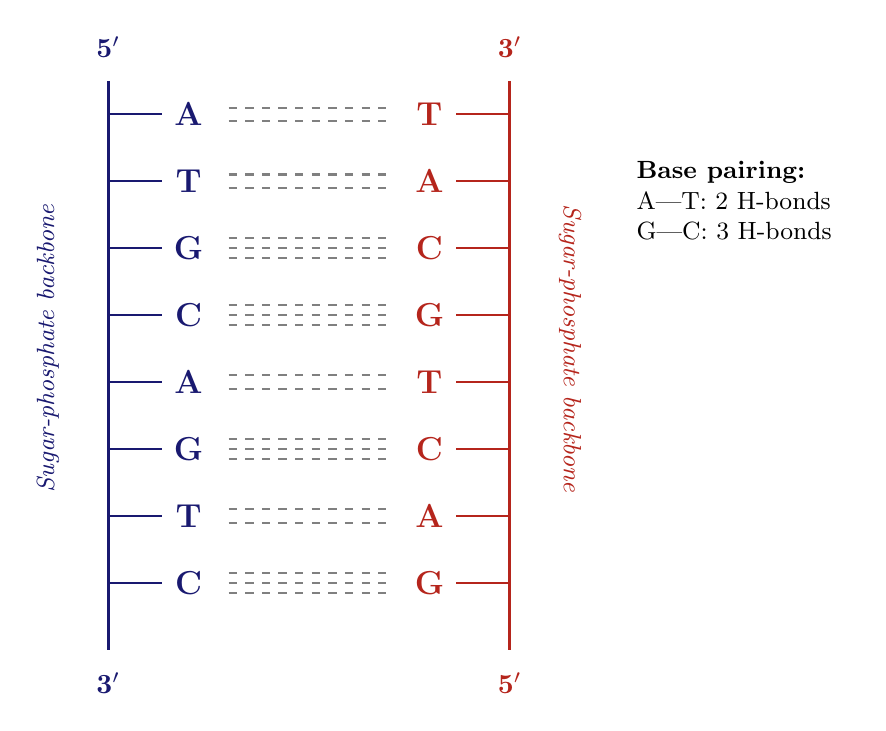
\begin{tikzpicture}[scale=0.85]
  % Draw the two backbone strands
  \draw[very thick, MidnightBlue] (0,0) -- (0,-8.5);
  \draw[very thick, BrickRed] (6,0) -- (6,-8.5);

  % Labels for strands
  \node[above, MidnightBlue, font=\bfseries] at (0,0.2) {5$'$};
  \node[below, MidnightBlue, font=\bfseries] at (0,-8.7) {3$'$};
  \node[above, BrickRed, font=\bfseries] at (6,0.2) {3$'$};
  \node[below, BrickRed, font=\bfseries] at (6,-8.7) {5$'$};

  % Base pairs
  \foreach \y/\leftbase/\rightbase/\bonds in {
    -0.5/A/T/2,
    -1.5/T/A/2,
    -2.5/G/C/3,
    -3.5/C/G/3,
    -4.5/A/T/2,
    -5.5/G/C/3,
    -6.5/T/A/2,
    -7.5/C/G/3
  } {
    % Base labels
    \node[MidnightBlue, font=\bfseries\large] at (1.2,\y) {\leftbase};
    \node[BrickRed, font=\bfseries\large] at (4.8,\y) {\rightbase};

    % Hydrogen bonds (dashed lines)
    \ifnum\bonds=2
      \draw[dashed, thick, gray] (1.8,\y+0.1) -- (4.2,\y+0.1);
      \draw[dashed, thick, gray] (1.8,\y-0.1) -- (4.2,\y-0.1);
    \else
      \draw[dashed, thick, gray] (1.8,\y+0.15) -- (4.2,\y+0.15);
      \draw[dashed, thick, gray] (1.8,\y) -- (4.2,\y);
      \draw[dashed, thick, gray] (1.8,\y-0.15) -- (4.2,\y-0.15);
    \fi

    % Connections from backbone to bases
    \draw[thick, MidnightBlue] (0,\y) -- (0.8,\y);
    \draw[thick, BrickRed] (6,\y) -- (5.2,\y);
  }

  % Sugar-phosphate backbone labels
  \node[rotate=90, MidnightBlue, font=\small\itshape] at (-0.9,-4) {Sugar-phosphate backbone};
  \node[rotate=-90, BrickRed, font=\small\itshape] at (6.9,-4) {Sugar-phosphate backbone};

  % Legend
  \node[anchor=north west, font=\small] at (7.5,-1) {
    \begin{tabular}{l}
    \textbf{Base pairing:} \\
    A---T: 2 H-bonds \\
    G---C: 3 H-bonds \\
    \end{tabular}
  };
\end{tikzpicture}
\caption[Simplified DNA structure.]{Simplified representation of DNA double-stranded structure showing the antiparallel sugar-phosphate backbones (blue and red) connected by complementary base pairs via hydrogen bonds (dashed lines). Note that G-C pairs have three hydrogen bonds, making them stronger than A-T pairs (two hydrogen bonds).}
\label{fig:molbio:dna-structure}
\end{figure}


% ============================================================
\section{DNA Organisation: From Double Helix to Chromosome}
\label{sec:molbio:dna-organisation}

The human genome contains approximately 3.2 billion base pairs of DNA. If stretched out, the DNA from a single human cell would be about 2 metres long. Yet it must fit inside a nucleus roughly 6 micrometres in diameter---a packing ratio of over 300,000 to 1. This remarkable feat of organisation is achieved through a hierarchy of packaging structures.

\subsection{Histones and Nucleosomes}
\label{subsec:molbio:nucleosomes}

The first level of packaging involves proteins called \textbf{histones}. DNA wraps around complexes of eight histone proteins (an \textbf{octamer} composed of two copies each of histones H2A, H2B, H3, and H4) to form structures called \textbf{nucleosomes}. Each nucleosome contains approximately 147 base pairs of DNA wrapped in 1.65 turns around the histone octamer, connected by short stretches of \textbf{linker DNA} (typically 20--60\basepair{}).

A fifth histone, \textbf{H1} (the linker histone), binds to the DNA as it enters and exits the nucleosome, helping to stabilise higher-order structures.

\subsection{Chromatin: Euchromatin and Heterochromatin}
\label{subsec:molbio:chromatin}

The chain of nucleosomes is called \textbf{chromatin}. Chromatin exists in two broad states:

\begin{itemize}[itemsep=2pt]
  \item \textbf{Euchromatin:} Loosely packed, ``open'' chromatin. Genes in euchromatic regions are generally accessible to the transcription machinery and may be actively expressed. Euchromatin appears light in electron microscopy.
  \item \textbf{Heterochromatin:} Tightly packed, ``closed'' chromatin. Genes in heterochromatic regions are generally silenced. Heterochromatin appears dark in electron microscopy. It can be further divided into:
  \begin{itemize}
    \item \textbf{Constitutive heterochromatin:} Permanently condensed regions, often found at centromeres and telomeres, typically containing repetitive sequences.
    \item \textbf{Facultative heterochromatin:} Regions that can switch between open and closed states depending on cell type or developmental stage. The inactive X chromosome in female mammals is a classic example.
  \end{itemize}
\end{itemize}

\subsection{Higher-Order Structures and Chromosomes}
\label{subsec:molbio:chromosomes}

Nucleosomes are further organised into higher-order structures. During cell division (mitosis or meiosis), chromatin condenses maximally into the dense, compact structures visible under a light microscope as \textbf{chromosomes}. Each chromosome consists of a single, continuous DNA molecule complexed with histones and other proteins.

Key chromosome structures include:
\begin{itemize}[itemsep=2pt]
  \item \textbf{Centromere:} The constricted region where the two sister chromatids are joined and where the spindle fibres attach during cell division.
  \item \textbf{Telomeres:} Repetitive DNA sequences (TTAGGG in humans) that cap the ends of chromosomes, protecting them from degradation and preventing them from fusing with neighbouring chromosomes.
\end{itemize}

\subsection{Ploidy}
\label{subsec:molbio:ploidy}

\textbf{Ploidy} refers to the number of complete sets of chromosomes in a cell. Most human somatic (body) cells are \textbf{diploid} (2n)---they contain two copies of each chromosome, one inherited from each parent. Human diploid cells have 46 chromosomes (23 pairs). Gametes (sperm and egg cells) are \textbf{haploid} (n), containing only 23 chromosomes. Some organisms, particularly plants, can be \textbf{polyploid} (e.g., wheat is hexaploid, with six copies of each chromosome), which adds complexity to genome assembly.

% TikZ: Chromatin organisation hierarchy
\begin{figure}[htbp]
\centering
\begin{tikzpicture}[
  level/.style={font=\small\bfseries},
  desc/.style={font=\scriptsize, text width=5.5cm},
  arrow/.style={-{Stealth[length=2.5mm]}, thick, gray},
  scale=0.9
]
  % Level 1: DNA double helix
  \node[level] (dna) at (0,0) {DNA Double Helix};
  \node[desc, right=0.5cm of dna] {$\sim$2\,nm diameter; base-pair level};
  \draw[very thick, MidnightBlue, decorate, decoration={snake, amplitude=1.5mm, segment length=4mm}]
    (-4,0) -- (-1.5,0);

  % Arrow down
  \draw[arrow] (0,-0.5) -- (0,-1.2);

  % Level 2: Nucleosome (beads on a string)
  \node[level] (nuc) at (0,-1.8) {Nucleosomes (``Beads on a String'')};
  \node[desc, right=0.5cm of nuc] {$\sim$11\,nm; 147\,bp wrapped around histone octamer};
  \foreach \x in {-4, -3, -2} {
    \draw[thick, MidnightBlue] (\x,-1.8) circle (0.3);
    \draw[thick, MidnightBlue, decorate, decoration={snake, amplitude=0.5mm, segment length=2mm}]
      (\x+0.3,-1.8) -- (\x+0.7,-1.8);
  }

  % Arrow down
  \draw[arrow] (0,-2.5) -- (0,-3.2);

  % Level 3: 30nm fibre
  \node[level] (fibre) at (0,-3.8) {Chromatin Fibre};
  \node[desc, right=0.5cm of fibre] {$\sim$30\,nm; nucleosomes packed together (debated structure)};
  \draw[very thick, OliveGreen, decorate, decoration={coil, amplitude=3mm, segment length=5mm}]
    (-4,-3.8) -- (-1.5,-3.8);

  % Arrow down
  \draw[arrow] (0,-4.5) -- (0,-5.2);

  % Level 4: Loops
  \node[level] (loop) at (0,-5.8) {Chromatin Loops};
  \node[desc, right=0.5cm of loop] {$\sim$300\,nm; loops anchored by CTCF/cohesin};
  \draw[very thick, Goldenrod] (-4,-5.8) to[out=60,in=120, looseness=1.8] (-2.5,-5.8);
  \draw[very thick, Goldenrod] (-2.5,-5.8) to[out=60,in=120, looseness=1.8] (-1,-5.8);

  % Arrow down
  \draw[arrow] (0,-6.5) -- (0,-7.2);

  % Level 5: Chromosome
  \node[level] (chr) at (0,-7.8) {Metaphase Chromosome};
  \node[desc, right=0.5cm of chr] {$\sim$1,400\,nm; maximally condensed during cell division};
  % Simple chromosome shape
  \draw[very thick, BrickRed, rounded corners=2pt]
    (-3.5,-7.2) -- (-3.5,-8.4) -- (-3.2,-8.4) -- (-3.2,-7.2) -- cycle;
  \draw[very thick, BrickRed, rounded corners=2pt]
    (-3.0,-7.2) -- (-3.0,-8.4) -- (-2.7,-8.4) -- (-2.7,-7.2) -- cycle;
  % Centromere
  \draw[very thick, BrickRed] (-3.5,-7.8) -- (-2.7,-7.8);
  \node[font=\tiny, BrickRed] at (-3.1,-8.7) {centromere};

\end{tikzpicture}
\caption[Chromatin organisation hierarchy.]{The hierarchy of DNA packaging from the naked double helix ($\sim$2\,nm) through nucleosomes ($\sim$11\,nm), chromatin fibres ($\sim$30\,nm), looped domains ($\sim$300\,nm), to the maximally condensed metaphase chromosome ($\sim$1,400\,nm). Each level of organisation has implications for gene regulation and is measurable by specific sequencing assays (e.g., \acrshort{ATAC-seq} for nucleosome positioning, \acrshort{Hi-C} for looping interactions).}
\label{fig:molbio:chromatin-hierarchy}
\end{figure}


% ============================================================
\section{Genes and the Genome}
\label{sec:molbio:genes-genome}

\subsection{What Is a Gene?}
\label{subsec:molbio:gene-definition}

A \textbf{gene} is a segment of DNA that contains the instructions for producing a functional product---usually a protein, but in some cases a functional RNA molecule. The human genome contains approximately 20,000--25,000 protein-coding genes, but these account for only about 1.5\% of the total genome. The rest---once dismissively called ``junk DNA''---includes regulatory sequences, non-coding RNAs, repetitive elements, and regions of unknown function.

\subsection{Gene Structure: Exons and Introns}
\label{subsec:molbio:exons-introns}

In eukaryotes, most protein-coding genes have a \textbf{split structure}: the coding sequence is divided into segments called \textbf{exons}, separated by non-coding sequences called \textbf{introns}. When the gene is transcribed, the entire region (exons + introns) is copied into a precursor RNA molecule (pre-mRNA). The introns are then removed through a process called \textbf{splicing}, and the exons are joined together to form the mature mRNA (see \cref{subsec:molbio:transcription}).

This arrangement allows for \textbf{alternative splicing}: different combinations of exons can be included in the final mRNA, producing different protein variants (called \textbf{isoforms}) from a single gene. Alternative splicing dramatically increases the diversity of proteins that can be produced from a finite number of genes. It is estimated that over 95\% of human multi-exon genes undergo alternative splicing.

\subsection{Regulatory Regions}
\label{subsec:molbio:regulatory-regions}

Genes do not exist in isolation---their expression is controlled by \textbf{regulatory DNA elements}:

\begin{description}[style=nextline, itemsep=3pt]
  \item[Promoter] A DNA sequence located immediately upstream (5$'${}) of the gene's transcription start site (TSS). The promoter is where \textbf{RNA polymerase} and general \textbf{transcription factors} bind to initiate transcription. Many promoters contain a TATA box (consensus sequence TATAAA) approximately 25--30\basepair{} upstream of the TSS, though many genes---particularly housekeeping genes---lack a TATA box and instead have CpG-island-associated promoters.

  \item[Enhancer] A regulatory DNA element that can increase transcription of a gene, often located thousands or even millions of base pairs away from the gene it regulates. Enhancers work by binding transcription factors and physically looping to contact the gene's promoter through three-dimensional chromatin folding. Enhancers can function regardless of their orientation or position relative to the gene.

  \item[Silencer] A regulatory element that represses transcription, functioning conceptually as the opposite of an enhancer.

  \item[Insulator] A boundary element that prevents regulatory signals (enhancers, silencers) from affecting genes on the other side of the insulator. The protein CTCF is a key component of many insulator elements.
\end{description}

\subsection{Repetitive Elements}
\label{subsec:molbio:repetitive-elements}

Approximately 45--50\% of the human genome consists of \textbf{repetitive elements}---DNA sequences present in many copies. Major categories include:

\begin{itemize}[itemsep=2pt]
  \item \textbf{SINEs (Short Interspersed Nuclear Elements):} The most common are Alu elements ($\sim$300\basepair{}), with over one million copies in the human genome.
  \item \textbf{LINEs (Long Interspersed Nuclear Elements):} The most common are LINE-1 (L1) elements ($\sim$6\kilobase{}), with about 500,000 copies.
  \item \textbf{DNA transposons:} ``Cut-and-paste'' mobile elements that are mostly inactive in the human genome.
  \item \textbf{Tandem repeats:} Including microsatellites (1--6\basepair{} repeat units, e.g., CACACA\ldots) and minisatellites (longer repeat units).
  \item \textbf{Segmental duplications:} Large blocks (>1\kilobase{}) of DNA that are duplicated, often in different locations in the genome.
\end{itemize}

\begin{warningbox}
Repetitive regions pose a major challenge for sequencing and genome assembly. Short sequencing reads originating from repetitive elements cannot be unambiguously placed in the genome, leading to ``multi-mapping'' reads and assembly gaps. Long-read sequencing technologies (\cref{ch:seqprinciples}) have significantly improved our ability to resolve repetitive regions.
\end{warningbox}

\subsection{Coding vs.\ Non-Coding DNA}
\label{subsec:molbio:coding-noncoding}

A common misconception is that most DNA ``does something'' by encoding proteins. In fact, the situation is far more nuanced:

\begin{itemize}[itemsep=2pt]
  \item $\sim$1.5\% of the human genome encodes protein sequences (exons of protein-coding genes).
  \item $\sim$5--10\% is estimated to be under evolutionary constraint (functional, including regulatory elements and non-coding RNAs), based on comparative genomics.
  \item $\sim$45--50\% consists of repetitive and transposable elements.
  \item The function (or lack thereof) of the remaining DNA is an active area of research.
\end{itemize}


% ============================================================
\section{The Central Dogma of Molecular Biology}
\label{sec:molbio:central-dogma}

In 1958, Francis Crick articulated what he called the \textbf{Central Dogma of molecular biology}: the principle that genetic information flows from DNA to RNA to protein. While we now know of exceptions and nuances (reverse transcription, RNA editing, prions), this framework remains the core organising principle of molecular biology.

% TikZ: Central Dogma diagram
\begin{figure}[htbp]
\centering
\begin{tikzpicture}[
  node distance=3.5cm,
  mol/.style={
    draw, rounded corners=6pt, thick,
    minimum width=2.8cm, minimum height=1.4cm,
    align=center, font=\large\bfseries
  },
  process/.style={font=\small\bfseries, fill=white, inner sep=2pt},
  arrow/.style={-{Stealth[length=4mm]}, very thick},
]
  % Molecules
  \node[mol, fill=MidnightBlue!15, draw=MidnightBlue] (dna) {DNA};
  \node[mol, fill=OliveGreen!15, draw=OliveGreen, right=of dna] (rna) {RNA};
  \node[mol, fill=BrickRed!15, draw=BrickRed, right=of rna] (protein) {Protein};

  % Main arrows
  \draw[arrow, MidnightBlue] (dna) -- node[process, above] {Transcription} (rna);
  \draw[arrow, OliveGreen] (rna) -- node[process, above] {Translation} (protein);

  % DNA replication (self-loop)
  \draw[arrow, MidnightBlue] (dna) to[out=150, in=210, looseness=4]
    node[process, left, xshift=-4mm] {Replication} (dna);

  % Reverse transcription (dashed)
  \draw[arrow, dashed, gray] (rna) to[out=210, in=-30]
    node[process, below, yshift=-2mm] {\color{gray}Reverse Transcription} (dna);

  % RNA replication (for RNA viruses)
  \draw[arrow, dashed, gray] (rna) to[out=30, in=-30, looseness=4]
    node[process, right, xshift=3mm] {\color{gray}RNA Replication} (rna);

\end{tikzpicture}
\caption[The Central Dogma of molecular biology.]{The Central Dogma: genetic information flows from DNA to RNA (transcription) to protein (translation). DNA can also be replicated. Dashed arrows indicate processes that occur in special contexts: reverse transcription (used by retroviruses and retrotransposons) and RNA-dependent RNA replication (used by some RNA viruses).}
\label{fig:molbio:central-dogma}
\end{figure}

The Central Dogma (\cref{fig:molbio:central-dogma}) describes three main processes:

\begin{enumerate}[itemsep=3pt]
  \item \textbf{Replication:} DNA $\rightarrow$ DNA. The faithful copying of the genome before cell division.
  \item \textbf{Transcription:} DNA $\rightarrow$ RNA. A gene's DNA sequence is copied into a messenger RNA (mRNA) molecule.
  \item \textbf{Translation:} RNA $\rightarrow$ Protein. The mRNA sequence is decoded by ribosomes to produce a chain of amino acids (a polypeptide) that folds into a functional protein.
\end{enumerate}


\subsection{Kinetics of Information Flow}
\label{subsec:molbio:kinetics}

The speed and fidelity of the enzymes that execute the Central Dogma are directly relevant to sequencing, because many sequencing chemistries harness these same enzymes (or engineered variants of them). \Cref{tab:molbio:polymerase-kinetics} summarises the key kinetic parameters.

\begin{table}[htbp]
\centering
\caption[Polymerase kinetics comparison.]{Kinetic parameters of the major polymerases involved in information flow. Processivity is the average number of nucleotides incorporated before the enzyme dissociates.}
\label{tab:molbio:polymerase-kinetics}
\small
\begin{tabularx}{\textwidth}{>{\bfseries}l X r r r}
\toprule
\textbf{Enzyme} & \textbf{Function} & \textbf{Speed (nt/s)} & \textbf{Error rate} & \textbf{Processivity} \\
\midrule
\species{E.~coli} DNA Pol III & Replication & 1,000 & $10^{-7}$ & $>$500,000 \\
\addlinespace
Human DNA Pol $\delta$ & Replication (lagging) & 30--50 & $10^{-7}$ & $\sim$500 \\
\addlinespace
Human DNA Pol $\varepsilon$ & Replication (leading) & 50--100 & $10^{-6}$--$10^{-7}$ & $>$10,000 \\
\addlinespace
Phi29 DNA Pol & Isothermal amplification & 25--50 & $10^{-6}$ & $>$70,000 \\
\addlinespace
\species{E.~coli} RNA Pol & Transcription & 40--80 & $10^{-4}$--$10^{-5}$ & $\sim$10,000 \\
\addlinespace
Human RNA Pol II & Transcription & 20--50 & $10^{-4}$--$10^{-5}$ & Variable \\
\addlinespace
Ribosome & Translation (aa/s) & 5--20 & $10^{-3}$--$10^{-4}$ & Complete mRNA \\
\bottomrule
\end{tabularx}
\end{table}

Several insights emerge from these kinetics:

\begin{itemize}[itemsep=2pt]
  \item \textbf{Replication is extraordinarily accurate.} After proofreading ($3' \rightarrow 5'$ exonuclease activity), replicative DNA polymerases achieve error rates of $\sim$$10^{-7}$ per base pair. With post-replication mismatch repair, the overall error rate drops to $\sim$$10^{-9}$--$10^{-10}$ per base pair per cell division.
  \item \textbf{Transcription is 100--1,000$\times$ less accurate} than replication. This is tolerable because (1) each transcript is temporary, (2) many copies of each mRNA are made, and (3) errors in any single transcript are diluted by the population.
  \item \textbf{Sequencing-by-synthesis co-opts polymerase chemistry.} The Phi29 polymerase (used in PacBio SMRT sequencing) combines high processivity ($>$70,000 nt) with moderate speed and good accuracy---ideal for long, continuous reads. Understanding these enzymatic parameters explains why different platforms achieve different read lengths and error rates.
\end{itemize}

\begin{keyconcept}[title={Fidelity Hierarchy}]
Information fidelity decreases at each step of the Central Dogma: DNA replication ($\sim$$10^{-10}$ errors/bp after repair) $>$ transcription ($\sim$$10^{-5}$ errors/nt) $>$ translation ($\sim$$10^{-4}$ errors/aa). This hierarchy reflects biological priorities: the genome must be copied with near-perfect fidelity across generations, while temporary RNA and protein errors are tolerable.
\end{keyconcept}


% ============================================================
\section{Transcription: From DNA to RNA}
\label{sec:molbio:transcription}

\textbf{Transcription} is the process of synthesising an RNA copy of a gene's DNA sequence. It is carried out by the enzyme \textbf{RNA polymerase}, which reads the template strand of DNA (3$'${} $\rightarrow$ 5$'${}) and synthesises a complementary RNA strand in the 5$'${} $\rightarrow$ 3$'${} direction.

\subsection{Transcription in Eukaryotes}
\label{subsec:molbio:euk-transcription}

Eukaryotic transcription is more complex than prokaryotic transcription and involves three main RNA polymerases:

\begin{itemize}[itemsep=2pt]
  \item \textbf{RNA Polymerase I:} Transcribes ribosomal RNA (rRNA) genes (except 5S rRNA).
  \item \textbf{RNA Polymerase II:} Transcribes messenger RNA (mRNA) and most non-coding RNAs, including miRNAs and lncRNAs. This is the polymerase most relevant to gene expression studies.
  \item \textbf{RNA Polymerase III:} Transcribes transfer RNAs (tRNAs), 5S rRNA, and other small RNAs.
\end{itemize}

The process of mRNA transcription by RNA Polymerase II occurs in three stages:

\begin{description}[style=nextline, itemsep=3pt]
  \item[Initiation] General transcription factors (TFIIA, TFIIB, TFIID, TFIIE, TFIIF, TFIIH) assemble at the promoter, forming the \textbf{preinitiation complex}. TFIID recognises and binds the TATA box (via its TBP subunit). RNA Polymerase II is recruited, and the DNA double helix is unwound (``melted'') at the transcription start site.

  \item[Elongation] RNA Polymerase II moves along the template strand, synthesising mRNA in the 5$'${} $\rightarrow$ 3$'${} direction. The RNA transcript is complementary to the template strand and identical in sequence to the coding (sense) strand, except that uracil (U) replaces thymine (T).

  \item[Termination] Transcription continues past the end of the coding sequence until specific termination signals are reached. In eukaryotes, the pre-mRNA is cleaved and polyadenylated (see below), and the polymerase dissociates from the DNA.
\end{description}

\subsection{mRNA Processing}
\label{subsec:molbio:mrna-processing}

In eukaryotes, the initial transcript (pre-mRNA) undergoes three critical processing steps before it can serve as a template for protein synthesis:

\begin{enumerate}[itemsep=3pt]
  \item \textbf{5$'${} Capping:} A modified guanine nucleotide (7-methylguanosine, m$^7$G) is added to the 5$'${} end of the pre-mRNA. The 5$'${} cap protects the mRNA from degradation, facilitates ribosome binding during translation, and aids in nuclear export.

  \item \textbf{Splicing:} Introns are removed and exons are joined together by a large ribonucleoprotein complex called the \textbf{spliceosome}. The spliceosome recognises specific sequences at intron--exon boundaries: the \textbf{5$'${} splice site} (donor site, typically GU), the \textbf{3$'${} splice site} (acceptor site, typically AG), and the \textbf{branch point} (an adenosine within the intron). As mentioned earlier, alternative splicing can produce different mRNA isoforms from the same gene.

  \item \textbf{3$'${} Polyadenylation:} A tail of 100--250 adenine nucleotides (the \textbf{poly-A tail}) is added to the 3$'${} end of the mRNA. The poly-A tail protects the mRNA from degradation, facilitates nuclear export, and aids in translation. In many \acrshort{RNA-seq} protocols, the poly-A tail is used to selectively capture mRNA from the total RNA pool (poly-A selection).
\end{enumerate}

\begin{tipbox}
The poly-A tail is exploited in many RNA sequencing library preparation protocols. Oligo-dT beads (short chains of thymine nucleotides) are used to capture mRNAs via their poly-A tails, enriching for mRNA and depleting abundant ribosomal RNA. However, this approach misses non-polyadenylated RNAs (such as many histone mRNAs and most non-coding RNAs). If your experiment aims to study non-coding RNAs, consider rRNA depletion instead of poly-A selection.
\end{tipbox}


% ============================================================
\section{Translation: From RNA to Protein}
\label{sec:molbio:translation}

\textbf{Translation} is the process by which the nucleotide sequence of an mRNA is decoded to produce a polypeptide (protein). This process takes place on \textbf{ribosomes}---complex molecular machines composed of ribosomal RNA (rRNA) and proteins.

\subsection{The Genetic Code}
\label{subsec:molbio:genetic-code}

The genetic code is the set of rules by which the nucleotide sequence of mRNA is translated into the amino acid sequence of a protein. The code is read in \textbf{triplets} called \textbf{codons}: each codon (a sequence of three nucleotides) specifies one amino acid or a stop signal.

Key properties of the genetic code:
\begin{itemize}[itemsep=2pt]
  \item \textbf{64 codons} encode 20 standard amino acids plus 3 stop signals. Because there are more codons than amino acids, the code is \textbf{degenerate} (redundant): most amino acids are specified by more than one codon.
  \item \textbf{AUG} (encoding methionine) serves as the \textbf{start codon}, signalling the beginning of translation.
  \item \textbf{UAA, UAG, UGA} are \textbf{stop codons}, signalling the end of translation.
  \item The code is nearly \textbf{universal}: the same codons specify the same amino acids in virtually all organisms, from bacteria to humans (with minor exceptions in mitochondria and a few organisms).
\end{itemize}

\subsection{The Process of Translation}
\label{subsec:molbio:translation-process}

Translation occurs in three phases:

\begin{description}[style=nextline, itemsep=3pt]
  \item[Initiation] The small ribosomal subunit binds to the mRNA and scans for the start codon (AUG). A special initiator tRNA carrying methionine base-pairs with the start codon. The large ribosomal subunit then joins to form the complete ribosome.

  \item[Elongation] The ribosome moves along the mRNA in the 5$'${} $\rightarrow$ 3$'${} direction, reading one codon at a time. For each codon, a \textbf{transfer RNA (tRNA)} molecule carrying the corresponding amino acid binds to the ribosome via complementary base pairing between the codon and the tRNA's \textbf{anticodon}. The amino acid is added to the growing polypeptide chain via a \textbf{peptide bond}.

  \item[Termination] When the ribosome reaches a stop codon, \textbf{release factors} bind and trigger the release of the completed polypeptide. The ribosome dissociates from the mRNA.
\end{description}

\subsection{Protein Folding and Function}
\label{subsec:molbio:protein-folding}

The newly synthesised polypeptide chain folds into a specific three-dimensional structure determined by its amino acid sequence. This folding occurs at multiple levels:

\begin{itemize}[itemsep=2pt]
  \item \textbf{Primary structure:} The linear sequence of amino acids.
  \item \textbf{Secondary structure:} Local folding patterns, mainly \textbf{alpha helices} and \textbf{beta sheets}, stabilised by hydrogen bonds.
  \item \textbf{Tertiary structure:} The overall three-dimensional shape of a single polypeptide, stabilised by hydrophobic interactions, hydrogen bonds, ionic bonds, and disulfide bridges.
  \item \textbf{Quaternary structure:} The arrangement of multiple polypeptide subunits into a multi-subunit complex (e.g., haemoglobin is a tetramer of four polypeptide chains).
\end{itemize}

A protein's function depends critically on its three-dimensional structure. Mutations that alter the amino acid sequence can disrupt folding and cause disease.


% ============================================================
\section{Types of RNA}
\label{sec:molbio:rna-types}

While mRNA is the most commonly studied RNA in sequencing experiments, cells produce a diverse array of RNA molecules with different functions:

\begin{description}[style=nextline, itemsep=3pt]
  \item[Messenger RNA (mRNA)] Encodes the amino acid sequence of proteins. Represents approximately 3--5\% of total cellular RNA by mass but is the most informationally diverse RNA class. This is the primary target of \acrshort{RNA-seq} experiments.

  \item[Ribosomal RNA (rRNA)] The catalytic and structural RNA component of ribosomes. Comprises approximately 80--85\% of total cellular RNA. In \acrshort{RNA-seq} experiments, rRNA is either depleted or excluded via poly-A selection; otherwise, the vast majority of reads would come from rRNA.

  \item[Transfer RNA (tRNA)] Small adapter molecules ($\sim$75--90 nucleotides) that carry amino acids to the ribosome during translation. Each tRNA has an anticodon that pairs with the corresponding mRNA codon.

  \item[MicroRNA (miRNA)] Small non-coding RNAs ($\sim$22 nucleotides) that regulate gene expression post-transcriptionally by binding to complementary sequences in the 3$'${} untranslated regions (3$'${} UTR) of target mRNAs, leading to mRNA degradation or translational repression. A single miRNA can regulate hundreds of target genes.

  \item[Long non-coding RNA (lncRNA)] Non-coding RNAs longer than 200 nucleotides with diverse roles in gene regulation, chromatin remodelling, and nuclear organisation. Examples include XIST (involved in X-chromosome inactivation) and HOTAIR (involved in chromatin remodelling). Thousands of lncRNAs have been identified, but the functions of most remain unknown.

  \item[Circular RNA (circRNA)] Covalently closed circular RNA molecules formed by back-splicing, in which a downstream splice donor joins to an upstream splice acceptor. circRNAs are resistant to exonucleolytic degradation and have been implicated as miRNA sponges, protein scaffolds, and regulators of transcription.

  \item[Piwi-interacting RNA (piRNA)] Small RNAs ($\sim$24--32 nucleotides) that interact with Piwi proteins and function primarily in transposon silencing in the germline.

  \item[Small nuclear RNA (snRNA)] Components of the spliceosome; essential for pre-mRNA splicing (e.g., U1, U2, U4, U5, U6 snRNAs).

  \item[Small nucleolar RNA (snoRNA)] Guide chemical modifications (methylation and pseudouridylation) of rRNA and other RNAs.
\end{description}

\begin{keyconcept}[title={RNA Diversity}]
The transcriptome is far more complex than just mRNA. Non-coding RNAs constitute the vast majority of cellular RNA and play critical roles in gene regulation, splicing, translation, and genome defence. Modern sequencing technologies can profile all of these RNA classes, but different library preparation methods are needed for different RNA types.
\end{keyconcept}


% ============================================================
\section{Epigenetics: Modifications Beyond the Sequence}
\label{sec:molbio:epigenetics}

\textbf{Epigenetics} refers to heritable changes in gene expression that occur without changes to the underlying DNA sequence. Epigenetic mechanisms control which genes are active in which cell types, and their dysregulation is implicated in cancer, developmental disorders, and ageing.

\subsection{DNA Methylation}
\label{subsec:molbio:dna-methylation}

\textbf{DNA methylation} is the addition of a methyl group ($-$CH$_3$) to the carbon-5 position of cytosine, producing \textbf{5-methylcytosine (5mC)}. In mammals, this modification occurs predominantly at \textbf{CpG dinucleotides}---positions where a cytosine is immediately followed by a guanine on the same strand.

Key points about DNA methylation:
\begin{itemize}[itemsep=2pt]
  \item \textbf{CpG islands:} Regions of the genome with a high density of CpG dinucleotides (typically >200\basepair{}, with observed/expected CpG ratio >0.6 and GC content >50\%). CpG islands are found at approximately 70\% of human gene promoters.
  \item \textbf{Gene silencing:} Methylation of CpG islands in promoter regions is generally associated with \textbf{transcriptional silencing}. Methylated promoters recruit proteins that compact chromatin, making genes inaccessible to the transcription machinery.
  \item \textbf{Maintenance and \textit{de novo} methylation:} DNA methyltransferase 1 (DNMT1) maintains methylation patterns during DNA replication by copying methyl marks from the parent strand to the newly synthesised strand. DNMT3A and DNMT3B establish new (``\textit{de novo}'') methylation patterns.
  \item \textbf{Demethylation:} Active demethylation involves oxidation of 5mC to 5-hydroxymethylcytosine (5hmC), 5-formylcytosine (5fC), and 5-carboxylcytosine (5caC) by TET (Ten-eleven translocation) enzymes, followed by base excision repair.
\end{itemize}

DNA methylation can be measured genome-wide using \acrshort{WGBS}, which treats DNA with sodium bisulfite to convert unmethylated cytosines to uracil (read as thymine after \acrshort{PCR}) while leaving methylated cytosines unchanged. This is discussed in detail in later chapters.

\subsection{Histone Modifications}
\label{subsec:molbio:histone-mods}

Histones are not merely passive spools for DNA packaging. The N-terminal ``tails'' of histone proteins protrude from the nucleosome and can be chemically modified at specific amino acid residues. These modifications---collectively called \textbf{histone marks}---influence chromatin structure and gene expression.

Major types of histone modifications include:

\begin{itemize}[itemsep=2pt]
  \item \textbf{Acetylation} (e.g., H3K27ac, H3K9ac): Addition of an acetyl group, generally associated with active gene expression. Acetylation neutralises the positive charge of lysine residues, loosening the interaction between histones and negatively charged DNA.
  \item \textbf{Methylation} (e.g., H3K4me3, H3K36me3, H3K27me3, H3K9me3): Addition of one, two, or three methyl groups to lysine or arginine residues. Unlike acetylation, methylation can be associated with either activation or repression, depending on the specific residue and the degree of methylation:
  \begin{itemize}
    \item H3K4me3 (trimethylation of lysine 4 on histone H3): marks \textit{active} promoters.
    \item H3K27me3: marks \textit{repressed} genes (Polycomb repression).
    \item H3K9me3: marks \textit{constitutive heterochromatin}.
    \item H3K36me3: marks \textit{actively transcribed} gene bodies.
  \end{itemize}
  \item \textbf{Phosphorylation} (e.g., H3S10ph): Addition of a phosphate group. Associated with chromosome condensation during mitosis and with transcriptional activation.
  \item \textbf{Ubiquitylation} (e.g., H2AK119ub, H2BK120ub): Addition of the small protein ubiquitin. Involved in both activation and repression.
\end{itemize}

The combination of histone modifications at a given genomic locus constitutes what is sometimes called the \textbf{histone code}---a complex regulatory layer that is read by effector proteins to control gene expression. These modifications can be mapped genome-wide using \acrshort{ChIP-seq} and related techniques (see later chapters).

\subsection{Chromatin Remodelling}
\label{subsec:molbio:chromatin-remodelling}

In addition to covalent modifications, chromatin structure is actively remodelled by \textbf{ATP-dependent chromatin remodelling complexes} (such as SWI/SNF, ISWI, CHD, and INO80 families). These enzymes use the energy of ATP hydrolysis to slide, eject, or restructure nucleosomes, thereby altering the accessibility of DNA to transcription factors and other regulatory proteins. Chromatin accessibility can be measured genome-wide using \acrshort{ATAC-seq} (see later chapters).

\begin{keyconcept}[title={The Epigenome as a Regulatory Layer}]
The epigenome---comprising DNA methylation, histone modifications, and chromatin accessibility---acts as a regulatory layer on top of the DNA sequence. It determines which genes are active in which cell types, without changing the genetic code itself. Every cell in your body (with rare exceptions) has the same genome, but different epigenomes are what make a neuron different from a liver cell. Modern sequencing technologies can map each of these epigenetic marks at single-nucleotide or single-cell resolution.
\end{keyconcept}


% ============================================================
\section{DNA Replication and Repair}
\label{sec:molbio:replication-repair}

\subsection{DNA Replication}
\label{subsec:molbio:replication}

Before a cell divides, it must duplicate its entire genome so that each daughter cell receives a complete copy. \textbf{DNA replication} is the process by which the double-stranded DNA molecule is copied. Key features include:

\begin{itemize}[itemsep=2pt]
  \item \textbf{Semi-conservative:} Each daughter DNA molecule contains one original (parental) strand and one newly synthesised strand. This was demonstrated by the famous Meselson--Stahl experiment in 1958.
  \item \textbf{Bidirectional:} Replication proceeds in both directions from each \textbf{origin of replication}. Eukaryotic genomes have thousands of origins to ensure the entire genome is replicated within the S phase of the cell cycle.
  \item \textbf{Key enzymes:}
  \begin{itemize}
    \item \textbf{Helicase:} Unwinds the double helix at the replication fork.
    \item \textbf{Primase:} Synthesises short RNA primers to provide a 3$'${}-OH group for DNA polymerase.
    \item \textbf{DNA polymerase:} Synthesises new DNA in the 5$'${} $\rightarrow$ 3$'${} direction, adding nucleotides complementary to the template strand. DNA polymerase cannot start synthesis \textit{de novo}---it can only extend an existing primer.
    \item \textbf{Ligase:} Joins Okazaki fragments on the lagging strand.
  \end{itemize}
  \item \textbf{Leading and lagging strands:} Because DNA polymerase can only synthesise in the 5$'${} $\rightarrow$ 3$'${} direction but the two template strands run antiparallel, replication is continuous on the \textbf{leading strand} (synthesised in the direction of fork movement) and discontinuous on the \textbf{lagging strand} (synthesised in short fragments called \textbf{Okazaki fragments} that are later joined).
  \item \textbf{Proofreading:} DNA polymerases have a 3$'${} $\rightarrow$ 5$'${} exonuclease activity that allows them to correct errors immediately, achieving an error rate of approximately one mistake per $10^{9}$--$10^{10}$ base pairs replicated.
\end{itemize}

\subsection{DNA Repair}
\label{subsec:molbio:repair}

DNA is constantly damaged by environmental factors (UV radiation, chemical mutagens) and by-products of normal metabolism (reactive oxygen species). Cells have evolved multiple DNA repair pathways:

\begin{itemize}[itemsep=2pt]
  \item \textbf{Mismatch repair (MMR):} Corrects base-pairing errors that escape proofreading during replication.
  \item \textbf{Base excision repair (BER):} Repairs small, non-helix-distorting lesions (e.g., oxidised or deaminated bases).
  \item \textbf{Nucleotide excision repair (NER):} Repairs bulky, helix-distorting lesions (e.g., thymine dimers caused by UV light).
  \item \textbf{Homologous recombination (HR):} Repairs double-strand breaks using the homologous chromosome or sister chromatid as a template. This is a high-fidelity repair mechanism.
  \item \textbf{Non-homologous end joining (NHEJ):} Repairs double-strand breaks by directly ligating the broken ends together. This is faster but more error-prone than HR, as it can introduce small insertions or deletions.
\end{itemize}

Defects in DNA repair pathways are associated with increased mutation rates and cancer predisposition. For example, mutations in BRCA1 and BRCA2 (which function in homologous recombination) dramatically increase the risk of breast and ovarian cancer.


% ============================================================
\section{Genetic Variation}
\label{sec:molbio:genetic-variation}

No two individuals (except identical twins) have exactly the same genome. The differences between individual genomes---collectively called \textbf{genetic variation}---are the raw material for evolution and the basis for individual traits, disease susceptibility, and pharmacological response. Understanding the types of genetic variation is essential for interpreting sequencing data.

\subsection{Single Nucleotide Polymorphisms (SNPs)}
\label{subsec:molbio:snps}

A \textbf{\acrfull{SNP}} is a position in the genome where a single nucleotide differs between individuals (or between the two copies of a chromosome within an individual). SNPs are the most common type of genetic variation. The human genome contains approximately 4--5 million SNPs per individual (compared to the reference genome), occurring roughly once every 600--1,000 base pairs.

Most SNPs have no functional consequence (they occur in non-coding, non-regulatory regions). However, some SNPs can:
\begin{itemize}[itemsep=2pt]
  \item Alter the amino acid sequence of a protein (missense variants).
  \item Create a premature stop codon (nonsense variants).
  \item Affect gene regulatory elements (eQTLs---expression quantitative trait loci).
  \item Influence splicing (splice site variants).
\end{itemize}

\subsection{Insertions and Deletions (Indels)}
\label{subsec:molbio:indels}

\textbf{\Acrfullpl{indel}} are genetic variants in which one or more nucleotides are inserted into or deleted from the genome. Short indels (1--50\basepair{}) are the second most common type of variation. Indels in protein-coding regions can cause \textbf{frameshift mutations} if their length is not a multiple of three, disrupting the reading frame of the gene and typically rendering the protein non-functional.

\subsection{Structural Variants (SVs)}
\label{subsec:molbio:svs}

\textbf{\Acrfullpl{SV}} are large-scale genomic alterations (typically defined as variants $>$50\basepair{}) that include:

\begin{itemize}[itemsep=2pt]
  \item \textbf{Deletions:} Loss of a segment of DNA.
  \item \textbf{Duplications:} Copying of a segment, resulting in extra copies.
  \item \textbf{Inversions:} Reversal of the orientation of a segment.
  \item \textbf{Translocations:} Transfer of a segment from one chromosome to another.
  \item \textbf{Complex rearrangements:} Combinations of the above.
\end{itemize}

Structural variants affect more total base pairs of the genome than SNPs and indels combined, yet they have historically been harder to detect because short sequencing reads often cannot span them. Long-read sequencing technologies have greatly improved SV detection.

\subsection{Copy Number Variants (CNVs)}
\label{subsec:molbio:cnvs}

\textbf{\Acrfullpl{CNV}} are a subtype of structural variant in which segments of the genome (typically >1\kilobase{}) are present in a variable number of copies. CNVs can encompass entire genes, leading to differences in gene dosage between individuals. Some CNVs are common and benign; others are associated with disease (e.g., the association between CNVs in the \gene{SMN1} gene and spinal muscular atrophy).

\begin{warningbox}
Different types of genetic variation require different sequencing strategies for reliable detection. \acrshort{SNP}s and short indels are well-detected by short-read \acrshort{WGS} at $\geq$30$\times$ coverage. Structural variants and CNVs often require long-read sequencing, linked-read sequencing, or specialised algorithms. No single method detects all variant types with equal sensitivity.
\end{warningbox}


% ============================================================
\section{Gene Regulation: Controlling When and Where Genes Are Expressed}
\label{sec:molbio:gene-regulation}

Not all genes are active in every cell. Gene expression is tightly regulated at multiple levels, from the accessibility of DNA to the stability of mRNA and protein. Understanding gene regulation is essential because many sequencing assays are specifically designed to measure different aspects of this regulation.

\subsection{Transcription Factors}
\label{subsec:molbio:tfs}

\textbf{Transcription factors (TFs)} are proteins that bind to specific DNA sequences (called \textbf{motifs} or \textbf{binding sites}) and activate or repress transcription. The human genome encodes approximately 1,500--1,600 transcription factors. They can be classified as:

\begin{itemize}[itemsep=2pt]
  \item \textbf{Activators:} Bind to enhancers or promoters and recruit co-activators and the transcription machinery, increasing transcription.
  \item \textbf{Repressors:} Bind to silencers or promoters and recruit co-repressors or block activator binding, decreasing transcription.
  \item \textbf{Pioneer factors:} A special class of transcription factors that can bind to closed (nucleosome-occupied) chromatin and initiate the opening process, enabling other factors to bind subsequently.
\end{itemize}

Transcription factor binding sites can be mapped genome-wide using \acrshort{ChIP-seq}, CUT\&RUN, or CUT\&Tag.

\subsection{Enhancers and Super-Enhancers}
\label{subsec:molbio:enhancers}

As described in \cref{subsec:molbio:regulatory-regions}, \textbf{enhancers} are distal regulatory elements that increase gene transcription. Key features:

\begin{itemize}[itemsep=2pt]
  \item Enhancers can be located tens of kilobases to megabases from the genes they regulate.
  \item They function by physically contacting promoters through \textbf{chromatin looping}.
  \item Active enhancers are typically marked by H3K27ac, H3K4me1, open chromatin (detectable by \acrshort{ATAC-seq}), and the presence of bound transcription factors.
  \item \textbf{Super-enhancers} are clusters of enhancers that drive high-level expression of genes important for cell identity. They are densely bound by transcription factors and the Mediator co-activator complex.
\end{itemize}

\subsection{Chromatin Accessibility and Gene Expression}
\label{subsec:molbio:chromatin-access}

The accessibility of DNA to transcription factors and RNA polymerase is a critical determinant of gene expression. Regions of \textbf{open chromatin} (depleted of nucleosomes) are more likely to be regulatory elements. Genome-wide maps of chromatin accessibility, obtained through \acrshort{ATAC-seq} or DNase-seq, provide a snapshot of the regulatory landscape of a cell.

\subsection{Post-Transcriptional Regulation}
\label{subsec:molbio:post-transcriptional}

Gene expression is also regulated after transcription:

\begin{itemize}[itemsep=2pt]
  \item \textbf{mRNA stability:} The half-life of mRNAs varies from minutes to hours. Regulatory elements in the 3$'${} UTR, as well as miRNA binding, influence mRNA degradation rates.
  \item \textbf{Translational regulation:} The rate at which ribosomes translate an mRNA can be regulated by upstream open reading frames (uORFs), RNA secondary structures, and RNA-binding proteins.
  \item \textbf{RNA modifications:} Chemical modifications of mRNA, such as N$^6$-methyladenosine (m$^6$A), affect mRNA stability, splicing, and translation. The study of these modifications is called \textbf{epitranscriptomics}.
\end{itemize}

\begin{keyconcept}[title={Multi-Level Gene Regulation}]
Gene expression is regulated at every step from DNA to functional protein: chromatin accessibility, transcription factor binding, transcription initiation and elongation, mRNA processing and splicing, mRNA export, mRNA stability, translation, and post-translational protein modification. Modern sequencing technologies can interrogate most of these levels, providing an unprecedented view of gene regulation.
\end{keyconcept}


% ============================================================
\section{Summary}
\label{sec:molbio:summary}

This chapter has covered the molecular biology essentials needed to understand sequencing technologies:

\begin{itemize}[itemsep=2pt]
  \item \textbf{Cells} come in two fundamental types: prokaryotic (no nucleus) and eukaryotic (membrane-bound nucleus and organelles).
  \item \textbf{DNA} is a double-stranded, antiparallel molecule composed of four nucleotides (A, T, G, C) held together by complementary base pairing.
  \item DNA is \textbf{packaged} into nucleosomes, chromatin, and chromosomes through a hierarchy of structures that influence gene expression.
  \item \textbf{Genes} are segments of DNA that encode functional products (proteins or RNAs), and their structure includes exons, introns, promoters, and enhancers.
  \item The \textbf{Central Dogma}---DNA $\rightarrow$ RNA $\rightarrow$ Protein---describes the flow of genetic information through transcription and translation.
  \item Cells produce many \textbf{types of RNA} beyond mRNA, including rRNA, tRNA, miRNA, lncRNA, and others, each with distinct functions.
  \item The \textbf{epigenome}---DNA methylation, histone modifications, and chromatin accessibility---provides a regulatory layer that controls gene expression without altering the DNA sequence.
  \item \textbf{Genetic variation}---SNPs, indels, structural variants, and CNVs---underlies individual differences in traits and disease susceptibility.
  \item \textbf{Gene regulation} operates at multiple levels, from chromatin structure to post-transcriptional processing.
\end{itemize}

With this foundation in place, we are ready to explore how modern sequencing technologies work at the chemical and physical level in \cref{ch:seqprinciples}.
